\documentclass[utf8,english]{gradu3}
% If you are writing a Bachelor's Thesis, use the following instead:
%\documentclass[utf8,bachelor,english]{gradu3}

\usepackage{graphicx} % for including pictures

\usepackage{amsmath} % useful for math (optional)

\usepackage{booktabs} % good for beautiful tables

\usepackage{csquotes}

% NOTE: This must be the last \usepackage in the whole document!
\usepackage[bookmarksopen,bookmarksnumbered,linktocpage]{hyperref}

\addbibresource{bibliography.bib} % The file name of your bibliography database 

\begin{document}

\title{Machine learning based automatic analysis of physics instruction quality}
\translatedtitle{Koneoppimispohjainen automaattinen fysiikan opetuksen laadun analyysi}
\studyline{Educational Technology}
\avainsanat{%
  TODO: Avainsanat}
\keywords{TODO: Keywords}
\tiivistelma{%
  TODO: Tiivistelmä
}
\abstract{%
  TODO: Abstract
}

\author{Aleksander Lempinen}
\contactinformation{\texttt{aleksander.lempinen@outlook.com}}
% use a separate \author command for each author, if there is more than one
\supervisor{Tommi Kärkkäinen}
\supervisor{Daniela Caballero}
\supervisor{Jouni Viiri}


% use a separate \supervisor command for each supervisor, if there
% is more than one

\maketitle

\begin{thetermlist}
\item[TODO] TODO: Glossary
\item[ASR] Automatic Speech Recognition
\item[KDD] Knowledge Discovery in Databases 
\item[HMM] Hidden Markov Model
\item[LSTM] Long Short-Term Memory 
\item[ML] Machine Learning
\item[NLP] Natural Language Processing
\item[RNN] Recurrent Neural Network
\item[NLTK] Natural Language ToolKit
\item[TF] Term Frequency
\item[TF-IDF] Term Frequency - Inverse Document Frequency 
\item[CAC] Corrected Arc Curve 
\end{thetermlist}

\mainmatter


%--------------------------------------------------------------------------------


\chapter{Introduction}

\emph{Automatic speech recognition (ASR)} has been one of the topics of interest in fields like computational linguistics and natural language processing, but more recently has expanded into more fields like education. This interest is sparked because of the increasing amount of audio speech data gathered in research activities such as observation or interviews. While speech-to-text ASR has been available for some time, further analysis of the text data in has remained a manual process especially in the domain of education. An important part of physics education is teaching students how to think like an expert and have deeper understanding of the physics concepts with monitoring and guidance of the instructor \parencite{wiemanTransformingPhysicsEducation2007}. Good physics instruction depends on the talk between the teacher and the students, which is called \emph{teacher talk} \parencite{scottTeachingScienceMeaningful2007}. Unfortunately teacher talk is not given the attention it deserves during teacher education \parencite{crespoPraisingCorrectingProspective2002,lehesvuoriDialogicTeachingScience2013}. 

Speech as data is sequential and messy in nature and requires cleaning and preprocessing before it can be used. In the case of teacher talk, it is traditionally analysed manually by researchers, which is a subjective and laborious process that is difficult to reproduce. Lack of analysis methods for teacher talk have been identified and new methods to analyse and visualize teacher talk during a lesson have been developed over time \parencite{viiriTeacherTalkPatterns2006,lehesvuoriVisualizingCommunicationStructures2013}. However, these methods rely on researchers first manually transcribing and coding the data, which is still laborious and difficult to reproduce. This is impractical for both research and for use in the field to give teachers feedback during their teacher education. Speech-to-text ASR is a well researched topic with significant advances especially in languages without a lot of speakers such as Finnish \parencite{kurimoModelingUnderresourcedLanguages2017}. Further processing of the text data is domain and application specific and not well researched in the case of teacher talk in science education and is the topic of this thesis. 

The problem is approached through a \emph{Knowledge Discovery in Databases (KDD)} process, which is an iterative process developed to extract valid, novel, potentially useful and understandable patterns from existing databases when manual data analysis is slow, expensive, highly subjective or otherwise impractical \parencite{fayyadKDDProcessExtracting1996}. KDD is a formal process that in addition to a \emph{data mining} step includes data preparation and interpretation and evaluation steps \parencite{fayyadKDDProcessExtracting1996}. This type of data analysis is exploratory in nature without assumptions and is used for automatic hypothesis generation, with emphasis on evaluation using quantitative measures \parencite{fayyadKDDProcessExtracting1996}.

The aim of this thesis is to automatically discover novel and potentially useful patterns from transcripts of teacher talk during physics lessons using data mining methods. 

The outcomes of this thesis are two contributions in analysing teacher talk:

\begin{itemize}
  \item Automatic visualization of teacher talk using concept networks
  %\item TODO motif discovery
\end{itemize}

%--------------------------------------------------------------------------------


\chapter{Physics instruction quality}
\label{chap:quip}

%TODO introduction to the chapter

\section{Teacher talk}
The quality of physics instruction has been at the centre of discussion, where traditional teaching methods have been criticized as inefficient at creating experts capable of thinking like physicists \parencite{wiemanTransformingPhysicsEducation2007}. The interaction between the teacher and the students is called \emph{teacher talk} and is a big part of all physics lessons, which is often taken for granted \parencite{scottTeachingScienceMeaningful2007}. Teacher talk is often not sufficiently addressed during teacher education and could be explained by the scarcity of available methods \parencite{lehesvuoriDialogicTeachingScience2013,viiriTeacherTalkPatterns2006, crespoPraisingCorrectingProspective2002}.

\section{Qualitative analysis of teacher talk}
Qualitative observation, where a mentor teacher makes observations during the lesson and gives feedback to the student teacher after the lesson, is an easy and a natural way to analyse teacher talk. According to Viiri and Saari \parencite*{viiriTeacherTalkPatterns2006} student teachers have issues with remembering what happened during the lesson and both self-reflection and teacher tutor feedback are based on memory and are unstructured. Therefore they developed a method to analyse teacher talk by visualizing talk types such as "teacher presentation", "authoritative discussion", "dialogic discussion", "peer discussion" and "other" of the lesson. This was achieved by first videotaping the lesson, manually transcribing it and then manually coding each time window into one of the teacher talk types. Viiri and Saari \parencite*{viiriTeacherTalkPatterns2006} point out that \enquote{Discourse analysis necessarily proceeds on the basis of the investigator’s interpretations of what was said.} This newly developed method is qualitative and subjective in nature by necessity.

This kind of qualitative and subjective analysis of teacher talk from classroom videos, usually by first transcribing or coding the talk based on some kind of a theoretical framework is not unique. For example Scott and Ametller \parencite*{scottTeachingScienceMeaningful2007} and Scott et al. \parencite*{scottPedagogicalLinkMaking2011} rely on small case studies and manual analysis of teacher talk from classroom video data either directly or from transcripts. The details of what they are looking for in the teacher talk is different in each case and dependent on the chosen theoretical framework and the research questions, but overall the process is similar. 

Figure \ref{fig:manualpipeline} represents a typical pipeline for analysis of teacher talk. First a meaningful representation is coded directly from transcriptions and classroom video. The representations are then visualized and interpreted or interpreted directly. Transcripts are often partial, because obtaining accurate transcriptions requires a lot of work and researchers will prefer to only transcribe some of the video and perform coding directly on the video. This type of coding is usually done by a single researcher. For example Jokiranta \parencite*{jokirantaNatureTeacherDiscourse2014} noted in her Master's thesis that the codings of the teacher talk data in her thesis were driven by research questions and literature and the analysis is based on the author's interpretation.

Qualitative analysis of teacher talk is not necessarily a weakness. Lehesvuori \parencite*{lehesvuoriDialogicTeachingScience2013} used a mix of qualitative and quantitative methods in his PhD dissertation and notes that qualitative methods of analysing teacher talk have allowed for more flexibility in contrast with quantitative methods, which were limited by the scarcity of dialogic interactions during the lessons. He identifies a weakness with quantitative methods of analysing teacher talk, which typically do not take into account the temporal aspect of teacher talk continuously changing during the lesson. Lehesvuori \parencite*{lehesvuoriVisualizingCommunicationStructures2013} also developed a method to visualize the teacher talk from classroom video of the lesson similar to Viiri and Saari \parencite*{viiriTeacherTalkPatterns2006} under a different theoretical framework.

\section{Quantitative analysis of teacher talk}
A more quantitative approach was used by Helaakoski and Viiri \parencite{helaakoskiContentContentStructure2014} to analyse the content structure of teacher talk. They used a relatively large dataset of classroom video consisting of 45 German, 28 Swiss and 25 Finnish lessons about \enquote{Relation  between  electrical  energy  and  power.} The videos were manually transcribed and from the videos and transcripts links between concept categories were identified and represented as a connectivity matrix, which could be visualized as a network of concepts. From the same connectivity other metrics and measures were computed. Helaakoski and Viiri \parencite*{helaakoskiContentContentStructure2014} found that \enquote{More  specifically,  the  frequencies  of  physics  concepts  and  connections  between  them  correlated  significantly  with  learning  gains.} This result is in line with previous research, which stresses the importance of paying attention to teacher talk. \parencite{viiriTeacherTalkPatterns2006,scottTeachingScienceMeaningful2007,scottPedagogicalLinkMaking2011}

%--------------------------------------------------------------------------------
\begin{figure}
  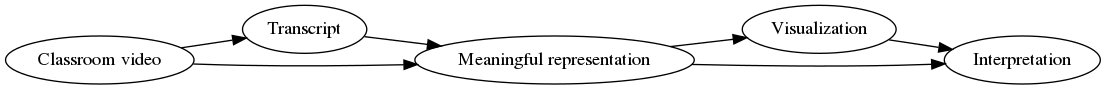
\includegraphics[width=\linewidth]{../figures/teacher_talk_manual_pipeline.png}
  \caption{Teacher talk analysis has a common manual pipeline. Classroom video is transcribed, meaningfully coded and then visualized and interpreted.}
  \label{fig:manualpipeline}
\end{figure}
%--------------------------------------------------------------------------------

In summary, teacher talk is an important component of any lesson that hasn't been sufficiently researched, because of a lack of good research methods. Specifically analysis of the temporal aspect of teacher talk during the lesson is interesting, but has few methods to analyse it. Improved methods to analyse teacher talk could lead to better feedback to student teachers and more opportunities for researching the interactions of the teacher during a lesson.

%--------------------------------------------------------------------------------


\chapter{Teacher talk as data}
\label{chap:speech}

%TODO: Introduction to the chapter

\section{Natural language processing}

Natural language processing as a field deals with applications of human language data, which is different from computational linguistics which focuses on studying human languages, but there is overlap and sharing of methods between the fields.

\subsection{Automatic speech recognition}
Automatic speech recognition (ASR) can be thought of as a subset of natural language processing. In fact, most ASR systems are speech-to-text, where any further processing is done with the text data. Speech might not always have clearly defined words and sentences, which shifts the focus from words to sounds called \emph{phonemes} and from sentences to word sequences called \emph{utterances}. Modelling conversational speech is especially difficult \parencite{kurimoModelingUnderresourcedLanguages2017}.

ASR is a classification task, where the goal is to predict what was said from the audio signal of speech. Early ASR systems had an acoustic model which detected phonemes to recognize numbers, some vowels and consonants for a single speaker \parencite{juangAutomaticSpeechRecognition2005}. Improvements in the acoustic model allowed for introduction of speaker-independent ASR \parencite{benzeghibaAutomaticSpeechRecognition2007,juangAutomaticSpeechRecognition2005}. The later addition of a language model based on statistical grammar and syntax helped more accurately predict the correct word based on what words previously appeared in the utterance \parencite{juangAutomaticSpeechRecognition2005}. Modern ASR systems utilize the fact that utterances are sequences of words and words are sequences of phonemes \parencite{bengioWordEmbeddingsSpeech2014}. 

Most commonly ASR is based on sequence models such as \emph{Hidden Markov Models (HMM)}, but deep learning approaches using \emph{Recurrent Neural Networks (RNN)} and \emph{Long Short-Term Memory (LSTM)} networks are gaining popularity for both acoustic models and language models or even end to end text-to-speech models \parencite{bengioWordEmbeddingsSpeech2014,enarviAutomaticSpeechRecognition2017}. Deep learning approach is more data-driven and relies on fewer assumptions, but instead requires more data for training \parencite{bengioWordEmbeddingsSpeech2014}. This might be impractical if training data is limited, which is often the case with languages without a lot of speakers such as Finnish. Depending on the architecture, an ASR system might be capable of either transcription, keyword spotting or both \parencite{juangAutomaticSpeechRecognition2005,enarviAutomaticSpeechRecognition2017}.

ASR is a difficult machine learning task because of a large search space, large vocabulary, undetermined length of word sequences and problems related to aligning speech signal to the text \parencite{enarviAutomaticSpeechRecognition2017}. Speech is highly variable even with a single speaker due to noise, but different pronunciations and accents mean that the audio signal will be different despite the same words being spoken \parencite{juangAutomaticSpeechRecognition2005}. Accents, dialects, emotional state, gender and casual speech slurring in spontaneous speech bring a lot of variation which makes conversational speech especially difficult compared to standard pronunciations and vocabulary \parencite{benzeghibaAutomaticSpeechRecognition2007, juangAutomaticSpeechRecognition2005}. Speaker-dependent systems are typically more accurate than speaker-independent systems \parencite{benzeghibaAutomaticSpeechRecognition2007,enarviAutomaticSpeechRecognition2017}.





\subsection{Text processing}


%TODO: NLP overview \parencite{silfverbergFinnPosOpensourceMorphological2016, kanervaTurkuNeuralParser2018}

%TODO: Definitions of concepts such as term, keyword, document, corpus and text

\subsection{Finnish language}
%TODO: Conversational vs official Finnish
Finnish language is particularly difficult for ASR because words are formed by concatenating smaller \parencite{enarviAutomaticSpeechRecognition2017}

%--------------------------------------------------------------------------------


\chapter{Methods}
%TODO Short introduction of the QUIP project


\section{KDD process}

According to Fayyaad et. al \parencite*{fayyadDataMiningKnowledge1996} traditional methods of manual analysis and interpretation rely on the person performing the analysis to be very familiar with the data and is a slow, expensive and highly subjective process. Even in the 90's they have noticed, that \enquote{manual data analysis is becoming completely impractical in many domains}. Because of the fast pace of accumulation of new data, they identified an urgent need for computational theories and tools to extract knowledge from data in at least a partially automatic way.

To address this a new field called Knowledge Discovery in Databases was introduced, that combines the fields of expert systems, machine learning, intelligent databases, knowledge acquisition, case-based reasoning and statistics \parencite{piatetsky-shapiroKnowledgeDiscoveryReal1990}. Originally KDD referred to the interactive and iterative process of extracting useful knowledge from data with emphasis on that knowledge is the end product of a data-driven discovery \parencite{fayyadKnowledgeDiscoveryData1996}. Data mining was a particular step in the process \parencite{fayyadKnowledgeDiscoveryData1996}, but later data mining and KDD became synonymous \parencite{piatetsky-shapiroKnowledgeDiscoveryDatabases2000}. A formal definition provided by Fayaad et. al \parencite*{fayyadKnowledgeDiscoveryData1996} is as follows:
\begin{displayquote}
Knowledge Discovery in Databases is the non-trivial process of identifying valid, novel, potentially useful, and ultimately understandable patterns in data.
\end{displayquote}

% How is KDD different from regular data analysis? TODO

% Importance of formulating the problem TODO

% Requirements/importances of KDD TODO
Found patterns should be novel, understandable, which are more subjective measures and valid on new data, which has more objective measures to evaluate them \parencite{fayyadKnowledgeDiscoveryData1996}. This evaluation is important, because knowledge discovery is based in statistics and patterns can be found even in random data \parencite{fayyadDataMiningKnowledge1996}.


The KDD process can be broken down into nine steps with iterations and loops possible between any two steps \parencite{fayyadKDDProcessExtracting1996,fayyadKnowledgeDiscoveryData1996,fayyadDataMiningKnowledge1996}:

\begin{enumerate}
  \item Understanding the domain
  \item Creating target dataset
  \item Data cleaning and preprocessing
  \item Data reduction and projection
  \item Matching goals to data mining method
  \item Exploratory data analysis
  \item Data mining
  \item Interpreting mined patterns
  \item Acting on discovered knowledge
\end{enumerate}

% Steps that are the focus of this thesis: preprocessing, data reduction & projection TODO

\section{Dataset}

%--------------------------------------------------------------------------------
\begin{table}[]
  \begin{tabular}{ | l | l | l |}
  \hline
  \textbf{Start} & \textbf{End}  & \textbf{Text} \\ \hline
  10.0 & 15.0 & hehkulamppua kakstoista tunteesta kirjottaas taas että miten tuo laske\\ \hline
  15.0 & 20.0 & virtapiirejä virtapiirejä rakettien kans vaikka kuinka paljon tähän\\
  \hline
  \end{tabular}
  \caption{The sometimes inaccurate transcript consists of start and end times of the split and the utterance spoken by the teacher during that split.}
  \label{table:transcript}
\end{table}
%--------------------------------------------------------------------------------


The dataset consists of audio recordings of Finnish physics teachers in comprehensive schools collected during the Quality of Physics Instruction study \parencite{fischerQualityInstructionPhysics2014,helaakoskiContentContentStructure2014}. Helaakoski and Viiri \parencite*{helaakoskiContentContentStructure2014} used microphones attached to 25 physics teachers to record lessons on the topic of \enquote{Relation between electrical energy and power}. Of the 25 teachers, 22 taught their topic in two 45 min lessons and 3 teachers taught their topic during a 90 minute double lesson. 

In addition to audio recordings from the teachers, the students were tested on the knowledge of the topic before and after the lesson and a list of physics keywords was obtained from a \enquote{FyKe 7-9 Fysiikka}\parencite{kangaskorteFyKeFysiikkaOPS2016} physics textbook glossary. The audio data was then automatically transcribed using AaltoASR in 5 second splits \parencite{hirsimakiImportanceHighOrderNGram2009} as shown in table ~\ref{table:transcript}. We will define a transcript as a \emph{document} and the full collection of transcripts as \emph{corpus} of documents.


% Dataset quality evaluation criteria

\section{Text Normalization}

%--------------------------------------------------------------------------------
\begin{table}[]
  \begin{tabular}{ | l | l | l | l | }
  \hline
  \textbf{Word} & \textbf{Snowball stem} & \textbf{Voikko lemma} & \textbf{Translation} \\ \hline
  virta & vir & Virta & current\\ \hline
  virtaa & virt & virrata & current\\ \hline
  virtapiiri & virtapiir & virtapiiri & electric circuit\\ \hline
  virtapiirejä & virtapiir & virtapiiri & electric circuits\\
  \hline
  \end{tabular}
  \caption{Both the Snowball stem and the Voikko lemma have problems with synonyms: the word "current" \emph{virtaa} is confused with the word "to flow" \emph{virrata} when lemma \emph{virta} was expected.}
  \label{table:stemmer}
\end{table}
%--------------------------------------------------------------------------------

First we apply text normalization techniques to the documents. First the documents are tokenized split by split into sequences of words using the NLTK tokenizer \parencite{birdNaturalLanguageProcessing2009}. Because of the agglutinative nature of Finnish, we then use the NLTK Snowball stemmer \parencite{birdNaturalLanguageProcessing2009} and the Voikko morphological analyser \parencite{pitkanenVoikkoFreeLinguistic2019}  for stemming and lemmatization. An example of the stems and lemmas obtained is shown in table ~\ref{table:stemmer}. We then process the physics keyword list in the same way. 

% Model evaluation criteria

\section{Bag-of-words}
A bag-of-words model is a simple way to represent a document as a feature. The basic idea is that for each token in the document we count the number of times the token occurred and represent it as a feature. For example two documents consisting of the sentences \enquote{the, pen, is, in, the, bag} and \enquote{a, pen, is, mightier, than, a, sword} would be represented like in table \ref{table:counts}. Other variations include using \emph{term frequency (TF)}, where the token count is divided by the total amount of tokens in the document to reduce the impact of differences in document length or \emph{term frequency - inverse document frequency (TF-IDF)}, where the term frequency is multiplied by inverse document frequency to reduce the impact of uninteresting words that commonly occur in many documents. 

Bag of words models create very large feature vectors with as many features as there are unique tokens in the corpus. With a large enough vocabulary the data is incredibly sparse with most of the tokens occurring zero times in a given document. This sparsity of the data can create problems further in the analysis pipeline, especially if there are few documents. To decrease the sparsity, we can combine the features into bins. A common technique is to combine the very rare tokens into an \enquote{other} feature and to remove very common tokens called \emph{stop words} that do not contain a lot of information such as \enquote{is, a , the, and, where}.

During experimentation we quickly noticed that it is necessary to reduce the amount of features. To do this we focus on the keyword list and combine tokens outside of the keyword list into an \emph{other} feature. This leaves us with a few hundred features instead of thousands of features. To reduce the amount of features even more, we bin the keywords into the following categories with the help of a physics expert: concepts, objects, units and meta keywords.

\begin{table}[]
  \begin{tabular}{ | l | l | l | l | l | l | l | l | l | l |}
    \hline
    \textbf{Document} & \textbf{a} & \textbf{bag} & \textbf{in} & \textbf{is} & \textbf{mightier} & \textbf{than} & \textbf{the} & \textbf{pen} & \textbf{sword}\\ \hline
    Document 1 & 0 & 1 & 1 & 1 & 0 & 0 & 2 & 1 & 0\\ \hline
    Document 2 & 1 & 0 & 0 & 1 & 1 & 1 & 0 & 1 & 1\\
    \hline
  \end{tabular}
  \caption{Example of bag of words with counts}
  \label{table:counts}
\end{table}

% Model evaluation criteria

\section{Token co-occurrence}

% Model evaluation criteria

\section{Concept network analysis}

Expanding upon the idea of visualizing concept structure using conceptual networks by Helaakoski and Viiri \parencite*{helaakoskiContentContentStructure2014}, we automatically generate weighted networks using the physics keyword list. In addition to obtaining a visualization of the content structure of the teacher talk during the lesson, we compute network measures to quantify the relationships between the concepts.

We first compute a physics concept co-occurrence matrix for each text normalized lesson using an overlapping window over the splits produced by the ASR system. Since a non-overlapping window would not count two concepts occurring together but in different windows as co-occurring, we count the co-occurrences within the first half of the window and then add the co-occurrences between the two halves. This is done to avoid counting the same co-occurrence within a window twice due to the overlapping window.

We then represent a pair of co-occurring physics concepts as nodes with the amount of co-occurrences as the weight for that edge. Using NetworkX \parencite{hagbergExploringNetworkStructure2008} we can visualize the lessons concept structure as a network of concepts as shown in figure %TODO.

% Model evaluating criteria

\section{Motif and discord discovery}
There are two main approaches to representing the temporal aspect of a lesson. The first approach would be to engineer more features, for example instead of computing a mean for the entire lesson we would split the lesson into smaller pieces called \emph{bins} and compute a separate mean for each bin. The second approach would be to have a sequence of examples, each representing a piece of the lesson. Such a sequence consisting of real umbers is called a time series \parencite{yehMatrixProfileVI2017}. Data mining and knowledge discovery of time series data involves techniques such as \emph{motif} discovery, \emph{discord} discovery, and \emph{segmentation} \parencite{yehUniversalTimeSeries2018}.

A motif is a pattern, where a sequence is repeating such as a heartbeat or an annual spike of sales before Christmas. On the other hand, a discord is a sequence that is different from the rest of the time series such as anomalies or black-swan events. More precisely, a motif is a pair of local subsequences that are very similar compared to the rest of the time series and a discord is a local subsequence that is very dissimilar compared to the rest of the time series \parencite{yehUniversalTimeSeries2018}. Semantic segmentation splits the time series into meaningful segments, where the patterns change. For example splitting a heartbeat time series into a "rest" and "run" segments.

Motif discovery, discord discovery and semantic segmentation can be done using an unsupervised technique called Matrix Profile \parencite{yehUniversalTimeSeries2018}. The basic idea of a Matrix Profile is to compute the smallest Euclidean distance of the local sequence to some other sequence elsewhere in the time series for each point in the time series. The result is that with only a parameter of window width we can obtain motifs that have the same low distance value, discords that are the peaks and have a large distance value and semantic segmentation that have few motifs spanning between the segments. There are three distinct ways to apply the Matrix Profile to analysing teacher talk.

The first way is to use the keyword frequency time series to compute a matrix profile for each lesson and use motif discovery to find patterns of similar local sequences within the same lesson. A \emph{corrected arc curve (CAC)} gives us the amount of motif pairs that cross each point. The lowest point of the CAC will have the fewest motifs spanning across it and it can be used to segment the lesson into two parts that have different patterns within them.

The second way is to append all keyword frequency time series into a single time series, compute the matrix profile and use motif discovery to find patterns of similar local sequences that can be between lessons or between different teachers. 

The third way is to have each lesson as a separate dimension and compute a multidimensional matrix profile and use motif discovery to find patterns that occur in the same point of the lesson across two or more lessons.

After the motif and discord discovery and semantic segmentation is completed, we visualize the matrix profile, CAC and the found patterns and interpret the local sequences. This interpretation phase is a manual process that relies on domain expertise and is necessary when using unsupervised techniques.

% Model evaluation criteria

\section{Cluster analysis}

% Unsupervised technique, based on a similarity measure, types of similarity measure

% Hierarchical clustering, AgglomerativeCLustering, Dendogram, linkage method

% Model evaluation criteria: CLuster validation indices, interpretation of the clusters


\section{Predictive modelling}

According to Shmueli \parencite*{shmueliExplainPredict2010} predictive modelling is defined as \enquote{the process of applying a statistical model or data mining algorithm to data for the purpose of predicting new or future observations}. This is in contrast to explanatory modelling, where causality provided by the theory is tested using statistical methods \parencite{shmueliExplainPredict2010}. It is important to point out, that explanatory modelling relies on \emph{construct operationalization}, that is tying theoretical constructs to observable measurements, but the predictive modelling does not \parencite{shmueliExplainPredict2010}. In other words, explanatory modelling aims to extract information about how nature associates inputs to outputs, while predictive modelling aims to use inputs to predict outputs \parencite{breimanStatisticalModelingTwo2001}.
% Supervised technique, example and label

% Decision tree

% Model evaluation criteria: validation, holdout set, k-fold, comparison to naive algorithms

\chapter{Results}



\section{Concept network analysis}

\begin{figure}
  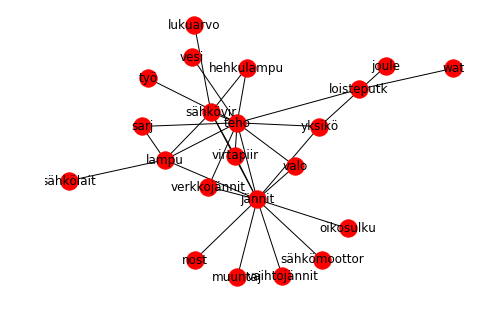
\includegraphics[width=\linewidth]{../figures/graph1.png}
  \caption{Concept network obtained from teacher talk during a Finnish physics lesson on the topic of }
  \label{fig:graph1}
\end{figure}

\section{Matrix profile}

% Example matrix profile and the found motifs, discords and segmentation using parameters X and Y TODO
An example of a matrix profile of a lesson is shown in figure TODO.

% Interpretation of the matrix profile motifs, discords and segmentation TODO

% Example of the same matrix profile, but with parameters A and B TODO

% Instability related to parameters and seemingly spurious patterns TODO

\section{Cluster analysis}

% Dendogram of the clusters, results of cluster validation indices TODO

% Interpretation of clusters TODO

% Example of dendogram and cluster validation indices with different parameters TODO

% Bad quality of the clusters, low cluster validation score TODO

\section{Predictive modelling}

% Chosen label and performance metric, results of the trained models using k-fold TODO

% Example of a decision tree TODO

% Bad model, comparison to naive random model TODO

\chapter{Related work}

Caballero et al. \parencite*{caballeroASRClassroomToday2017} applied ASR and NLP techniques to analyse teacher talk in Spanish and Finnish in a pilot study to determine the feasibility of the approach and maturity of modern ASR systems. Two teachers were equipped with microphones and concept networks were created and visualized by counting which physics concept keywords occurred together in the teacher's talk. We expanded upon this idea by using a larger dataset with more teachers, using alternative NLP methods such as lemmatization in addition to stemming, adding more representations of the data and including taking the temporal aspect of the lesson into account in the analysis and visualizations.

Fan et al. \parencite*{fanCourseMIRROREnhancingLarge2015} used NLP techniques to improve interactions between the student and the instructor. They developed a pilot system to collect self-reflections from the students, summarize them using NLP and then show the summaries to the instructors through a graphical interface. We believe that a simple to use interface to show summaries is necessary for teachers and developed visualizations so that teachers can see the content structure of the entire lesson at a glance.

% Find more related work TODO

\chapter{Discussion}

% partial success of word co-occurrence: network analysis
% Failure of bag of words: matrix profiles, clustering and decision trees

% interpretation of found patterns

% Acting on discovered knowledge


% Limitations TODO

% Ethics and privacy
In addition to the ethics of data collection in a classroom setting and potential misuse, automatic processing of teacher talk could be used for teacher assessment which is not based in pedagogical theory. The methods described in this thesis are based on potentially useful patterns in the data and further confirmatory research is required to determine whether the patterns are indeed useful.

\chapter{Conclusions}




%TODO Further research

%TODO Acknowledgements
Research was done in collaboration with the Department of Teacher Education at University of Jyväskylä and Centro de Investigación Avanzada en Educación (CIAE) at University of Chile.
 
\printbibliography

\end{document}
